\documentclass[a4paper]{article}

\usepackage{hyperref}
\usepackage{listings}
\usepackage{paralist}
\usepackage{siunitx}
\usepackage{graphicx}
\usepackage{epstopdf}
\usepackage{color}

\definecolor{mygray}{rgb}{0.4,0.4,0.4}
\definecolor{mygreen}{rgb}{0,0.8,0.6}
\definecolor{myorange}{rgb}{1.0,0.4,0}

\lstset{frame = none,
    basicstyle=\footnotesize\sffamily\color{black},
    frame = single,
    numbers = none,
    numberfirstline = false,
    language = python,
    basicstyle = \ttfamily,
    stringstyle=\color{myorange},
    keywordstyle=\color{mygreen},
    numberstyle=\tiny\color{mygray},
    commentstyle=\color{mygray}
}
\usepackage{listings}

\begin{document}
    \title{Security Engineering Cipher Design Execise}
    \author{Elias Trommer, Matthias Pollach, Moritz Schaefer}
    \maketitle
    \begin{abstract}
	In this paper, we will propose a design of cipher that is based on a feistel structure and is supposed to provide improved resistance against differential attacks
    \end{abstract}
	%\tableofcontents
    \section{General Design Principles}
        \begin{figure}[h!]
	\centering
	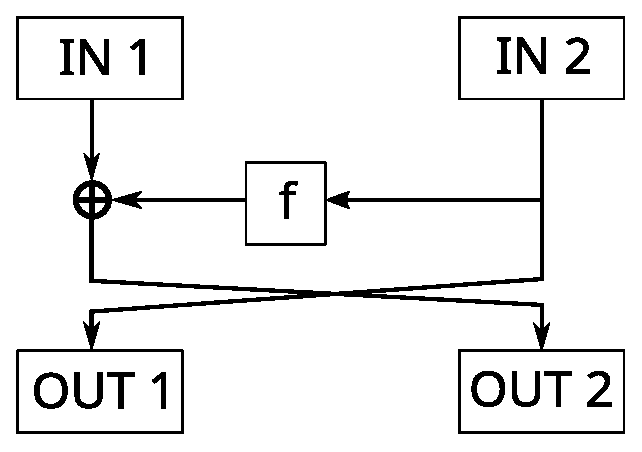
\includegraphics[scale=.4]{feistelstruc.eps}
	\caption{Feistel Structure}
	\label{fig:feistel}
    \end{figure}
 We chose the basic principle of the feistel cipher, as it provides E/D similarity without alterations in the process and relies heavily on XOR operations which can easily be implemented in hardware.\\[0.5em]
    Our cipher uses a block size of 128bit with a 256bit key over 20 rounds. 
    \section{Round Function}
	The round function is that of a regular feistel cipher with two blocks of input from the plaintext, one of which is transformed through the Feistel function and XORed to the other plain text block. After each round both blocks are exchanged for a total of 20 rounds.
    \section{Feistel function}
        \begin{figure}[t]
	\centering
	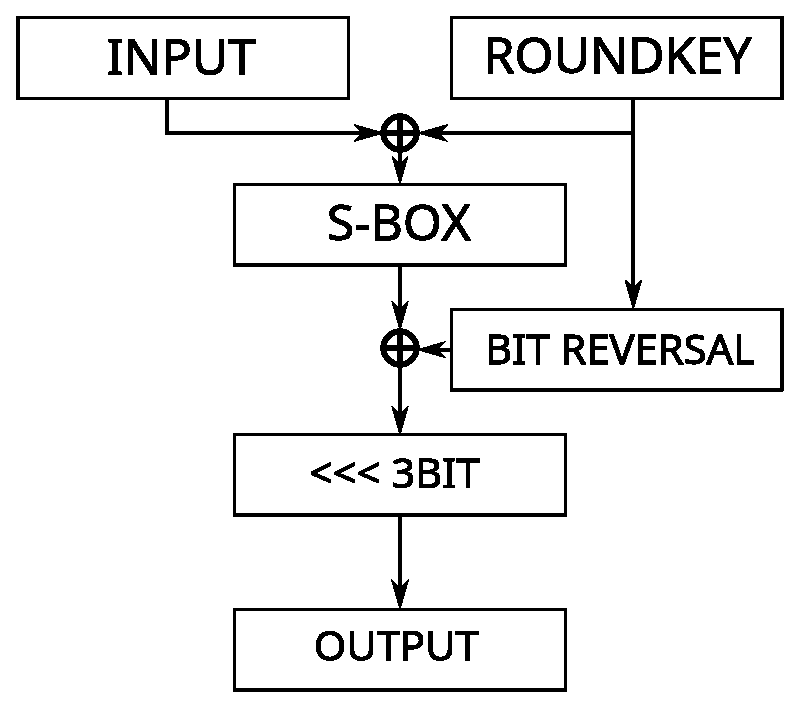
\includegraphics[scale=.4]{roundfun.eps}
	\caption{Proposed Feistel Function}
	\label{fig:roundfun}
    \end{figure}
The round function takes a 64bit plaintext block and the round key as an input which are XORed to form the input to the S-Box which provides non-linearity. The S-Box output is again XORed with the mirrored (LSB $\rightarrow$ MSB) roundkey. Then a permutation is applied by rotating the result by 3 bits for additional diffusion. 3 bits have been chosen because the provide the very little overlap between original blocks through the rounds
    \section{S-Box Design}
\begin{table}[h]
    \tabcolsep = 0.08cm
    \begin{tabular}{|r|rrrrrrrrrrrrrrrr|}
	\hline
	 & 0 & 1 & 2 & 3 & 4 & 5 & 6 & 7 & 8 & 9 & A & B & C & D & E & F \\ \hline
	 0 & 93 & 6B & E5 & 8B & E & C4 & 68 & C & 3 & 76 & 52 & 46 & C & 7F & B9 & 63 \\ 
	 1 & 33 & 8B & 27 & C3 & AA & B1 & 0 & 8 & C9 & 2 & EC & DB & 38 & D5 & 8D & A8 \\ 
	 2 & 12 & 4C & 31 & 47 & AF & 9E & 41 & 7C & EA & D4 & B9 & 2F & 85 & 4 & 72 & 57 \\ 
	 3 & 49 & 53 & 47 & 4B & 9E & AB & 9D & 16 & D1 & 52 & DE & AB & C1 & 26 & 46 & 89 \\ 
	 4 & FA & 88 & 5E & 2D & BD & CE & 1D & 41 & 48 & 86 & B5 & E0 & 14 & 16 & 4E & 65 \\ 
	 5 & 58 & 2B & C5 & DE & 4D & D4 & 7D & AB & 7B & 1A & A5 & 39 & 26 & EE & 4D & BB \\ 
	 6 & A5 & FE & 14 & 8 & 40 & B8 & 15 & C2 & D8 & 9 & A4 & F5 & 95 & A & 1F & D2 \\ 
	 7 & 40 & 74 & 7A & AC & 19 & 89 & 55 & C3 & 32 & D6 & CA & E1 & DF & CB & A2 & A5 \\ 
	 8 & AE & F6 & 8C & 21 & 41 & C & 8B & 42 & C & DA & 4C & D5 & 6D & 21 & E3 & 34 \\ 
	 9 & A7 & 4A & D1 & D1 & C2 & DF & EF & 51 & 96 & D5 & 15 & 1A & B2 & 3C & 7A & 10 \\ 
	 A & 2D & 16 & 45 & 99 & D1 & 4E & DF & DB & 19 & BC & 52 & 2F & 99 & 7C & B5 & C4 \\ 
	 B & A7 & A3 & 4E & 69 & 7D & 5F & F6 & EA & 1D & D7 & EB & B3 & 10 & 6A & 8C & 9C \\ 
	 C & A & E7 & 9A & C8 & AD & 6 & 69 & 8A & 34 & DA & F1 & 8F & 8C & B4 & A3 & F0 \\ 
	 D & 14 & F8 & BD & 5F & 32 & BF & 5C & D0 & D5 & E1 & 80 & 8A & BC & D2 & 32 & D0 \\ 
	 E & 96 & 13 & 9A & 9E & 12 & ED & CE & EE & B8 & C7 & 39 & F & 87 & 68 & 52 & 90 \\ 
	 F & E2 & 71 & 18 & 84 & B7 & DF & 6F & 85 & A6 & 63 & 75 & C7 & 2F & 90 & 40 & 90 \\ 
	 \hline
     \end{tabular}
     \caption{Proposed S-Box Design (HEX formated)}
     \label{sbox}
 \end{table}
    The S-Box provides the non-linearity of the system. It has an input of 8bits and an output of 8bit and is based on a pseudo-random distribution generated by an exponential function which is part of the implementation and can therefore be precomputed. The functions takes the upper and lower nibble of the input as x and y components. The generating function chosen is
$$
S(x,y) = \mathrm{round} \left( \frac{\exp \left(3(x+1) + 17(y+3)\right)}{9} \right) \bmod 256
$$
Both components are added with a bias and multiplied by different prime numbers to achieve a high spreading of the expected values of the exponential function. The scaling factor 9 is necessary to be able to compute the S-Box with 64bit floating point numbers. For each combination of inputs the output of the S-Box can be found in~\ref{sbox}.
\subsection{Differential Properties}
Differential analysis of the proposed S-Box can be conducted automatically by the following piece of code:
\begin{lstlisting}
diffs = dict([ (i, [0]*256) for i in range(256) ])
for a,b in itertools.product(range(256), range(256))
diff = s_box[a&0x0f,a>>4] ^ s_box[b&0x0f,b>>4]
diffs[a^b][diff] += 1
\end{lstlisting}
Evaluation of the generated output shows, that there are only two differential input-output combinations that occur more than ten times, and no combination occurs more than twelve times. Considering the size of the S-Box, these differential properties are satisfying, as it is not easy for an attacker to find a large amount of pairs with the same differential characteristics.
\section{Key Schedule}
The subkey for each of the 20 rounds are generated from the master key $K$ by the following set of rules:
\begin{itemize}
    \item The 256bit key is split into 4 parts of 64bits each. These parts provide the round keys for four rounds
    \item after 4, 8 and 16 rounds the master key is rotated by 101 bits to provide a good overlap of the key parts through several rounds
    \item after rotation, we add a constant to the master key from the last 4 rounds: $$K_{4n+1} = K_{4n} + 1 + 2^{64} + 2^{128} + 2^{192}$$ which in simpler words means, that the constant $1$ is added to each subkey to reduce problems with weak keys.
\end{itemize}
\end{document}
